\newcommand{\figuraComparacionPlacas}{%
\begin{figure}[H]
    \centering
    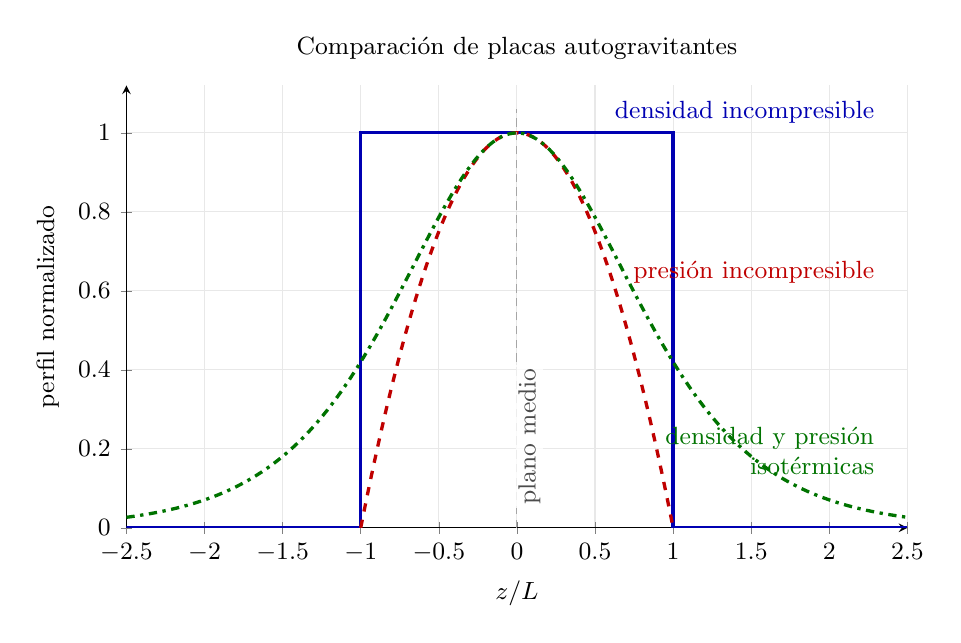
\begin{tikzpicture}[font=\small]
        \begin{axis}[
            width=11.5cm,
            height=7.2cm,
            xmin=-2.5,xmax=2.5,
            ymin=0,ymax=1.12,
            axis lines=left,
            xlabel={$z/L$},
            ylabel={perfil normalizado},
            title={Comparación de placas autogravitantes},
            grid=major,
            grid style={gray!18}]

            \addplot[very thick,blue!70!black]
                coordinates {(-2.5,0) (-1,0) (-1,1) (1,1) (1,0) (2.5,0)};

            \addplot[very thick,red!75!black,dashed,domain=-1:1,samples=120]
                {1-x^2};

            \addplot[very thick,green!45!black,dash dot,domain=-2.5:2.5,samples=180]
                {1/(cosh(x)^2)};

            \node[blue!70!black,anchor=south east]
                at (axis cs:2.35,1.00) {densidad incompresible};
            \node[red!75!black,anchor=north east]
                at (axis cs:2.35,0.70) {presión incompresible};
            \node[green!45!black,anchor=north east,align=right]
                at (axis cs:2.35,0.28) {densidad y presión\\isotérmicas};

            \draw[densely dashed,gray!70]
                (axis cs:0,0)--(axis cs:0,1.06);
            \node[anchor=west,rotate=90,text=black!70,fill=white,
                  fill opacity=0.8,text opacity=1,inner sep=1pt]
                at (axis cs:0.08,0.05) {plano medio};
        \end{axis}
    \end{tikzpicture}
    \caption{La placa incompresible tiene densidad uniforme y presión
    parabólica dentro de un espesor finito. En la placa isotérmica, tanto la
    densidad como la presión decrecen suavemente con un perfil
    $\operatorname{sech}^2$.}
    \label{fig:comparacion-placas}
\end{figure}%
}